\documentclass{article}\usepackage[]{graphicx}\usepackage[]{color}
% maxwidth is the original width if it is less than linewidth
% otherwise use linewidth (to make sure the graphics do not exceed the margin)
\makeatletter
\def\maxwidth{ %
  \ifdim\Gin@nat@width>\linewidth
    \linewidth
  \else
    \Gin@nat@width
  \fi
}
\makeatother

\definecolor{fgcolor}{rgb}{0.345, 0.345, 0.345}
\newcommand{\hlnum}[1]{\textcolor[rgb]{0.686,0.059,0.569}{#1}}%
\newcommand{\hlstr}[1]{\textcolor[rgb]{0.192,0.494,0.8}{#1}}%
\newcommand{\hlcom}[1]{\textcolor[rgb]{0.678,0.584,0.686}{\textit{#1}}}%
\newcommand{\hlopt}[1]{\textcolor[rgb]{0,0,0}{#1}}%
\newcommand{\hlstd}[1]{\textcolor[rgb]{0.345,0.345,0.345}{#1}}%
\newcommand{\hlkwa}[1]{\textcolor[rgb]{0.161,0.373,0.58}{\textbf{#1}}}%
\newcommand{\hlkwb}[1]{\textcolor[rgb]{0.69,0.353,0.396}{#1}}%
\newcommand{\hlkwc}[1]{\textcolor[rgb]{0.333,0.667,0.333}{#1}}%
\newcommand{\hlkwd}[1]{\textcolor[rgb]{0.737,0.353,0.396}{\textbf{#1}}}%
\let\hlipl\hlkwb

\usepackage{framed}
\makeatletter
\newenvironment{kframe}{%
 \def\at@end@of@kframe{}%
 \ifinner\ifhmode%
  \def\at@end@of@kframe{\end{minipage}}%
  \begin{minipage}{\columnwidth}%
 \fi\fi%
 \def\FrameCommand##1{\hskip\@totalleftmargin \hskip-\fboxsep
 \colorbox{shadecolor}{##1}\hskip-\fboxsep
     % There is no \\@totalrightmargin, so:
     \hskip-\linewidth \hskip-\@totalleftmargin \hskip\columnwidth}%
 \MakeFramed {\advance\hsize-\width
   \@totalleftmargin\z@ \linewidth\hsize
   \@setminipage}}%
 {\par\unskip\endMakeFramed%
 \at@end@of@kframe}
\makeatother

\definecolor{shadecolor}{rgb}{.97, .97, .97}
\definecolor{messagecolor}{rgb}{0, 0, 0}
\definecolor{warningcolor}{rgb}{1, 0, 1}
\definecolor{errorcolor}{rgb}{1, 0, 0}
\newenvironment{knitrout}{}{} % an empty environment to be redefined in TeX

\usepackage{alltt}[12pt]
\usepackage{Sweave}
\usepackage{float}
\usepackage{graphicx}
\usepackage{tabularx}
\usepackage{siunitx}
\usepackage{amssymb} % for math symbols
\usepackage{amsmath} % for aligning equations
\usepackage{mdframed}
\usepackage{natbib}
\bibliographystyle{..//bib/styles/gcb}
\usepackage[hyphens]{url}
\usepackage[small]{caption}
\setlength{\captionmargin}{30pt}
\setlength{\abovecaptionskip}{0pt}
\setlength{\belowcaptionskip}{10pt}
\topmargin -1.5cm        
\oddsidemargin -0.04cm   
\evensidemargin -0.04cm
\textwidth 16.59cm
\textheight 21.94cm 
%\pagestyle{empty} %comment if want page numbers
\parskip 7.2pt
\renewcommand{\baselinestretch}{2}
\parindent 0pt
\usepackage{lineno}
\linenumbers
\usepackage{setspace}
\doublespacing

\newmdenv[
  topline=true,
  bottomline=true,
  skipabove=\topsep,
  skipbelow=\topsep
]{siderules}

%% R Script


\IfFileExists{upquote.sty}{\usepackage{upquote}}{}
\begin{document}
\noindent \textbf{\Large{Heightened false spring risk with climate change across six European tree species \\
OR \\
False spring risk increases across European trees in the face of climate change \\
OR \\
Climate change increases the risk of false springs in European trees}}

\noindent Authors:\\
C. J. Chamberlain $^{1,2}$, B. I. Cook $^{3}$, I. Morales Castilla $^{1,4}$ \& E. M. Wolkovich $^{1,2,5}$
\vspace{2ex}\\
\emph{Author affiliations:}\\
$^{1}$Arnold Arboretum of Harvard University, 1300 Centre Street, Boston, Massachusetts, USA; \\
$^{2}$Organismic \& Evolutionary Biology, Harvard University, 26 Oxford Street, Cambridge, Massachusetts, USA; \\
$^{3}$NASA Goddard Institute for Space Studies, New York, New York, USA; \\
$^{4}$Edificio Ciencias, Campus Universitario 28805 Alcal\'{a} de Henares, Madrid, Spain \\
$^{5}$ Forest \& Conservation Sciences, Faculty of Forestry, University of British Columbia, 2424 Main Mall, Vancouver, BC V6T 1Z4\\
\vspace{2ex}
$^*$Corresponding author: 248.953.0189; cchamberlain@g.harvard.edu\\

\renewcommand{\thetable}{\arabic{table}}
\renewcommand{\thefigure}{\arabic{figure}}
\renewcommand{\labelitemi}{$-$}
\setkeys{Gin}{width=0.8\textwidth}

%%%%%%%%%%%%%%%%%%%%%%%%%%%%%%%%%%%%%%%%%%%%%%%
%%%%%%%%%%%%%%%%%%%%%%%%%%%%%%%%%%%%%%%%%%%%%%%

%%%%%%%%%%%%% 9 May 2019 - Cat - Made a lot of updates. Need to reread entirely but start back up at line 168 first %%%%%%%%%%%%%%%%%%

\section*{Abstract}
%Temperate and boreal forests have always been at risk of late spring freezing events -- also known as false springs -- but with climate change it is unclear whether these events will continue to pose a threat. There is growing interest in false springs, which has lead to diverging evidence: some studies have found false springs are increasing with climate change while others are finding the reverse or even no change in frequency. There are many regional factors that contribute to a plants risk of a false spring but, to date, no study has compared all of these regional and climatic factors at once. 
Using PEP725 leafout data for six tree species across 11,648 sites in Europe, we assessed the effects of the North Atlantic Oscillation (NAO), mean spring temperature, elevation and distance from the coast to determine which were the strongest predictors of false spring risk and how these predictors shifted with climate change. False spring risk varied across the six species but, overall, false spring risk is increasing with climate change across both early and late bud bursting species. Mean spring temperature and distance from the coast were the strongest predictors of false spring risk, with higher mean spring temperatures having fewer false springs and sites further from the coast experiencing more false springs. Our results suggest that considering multiple spatial and climatic factors is essential for predicting false spring risk --- especially as these events are increasing with climate change.

\section*{Introduction}
Temperate tree and shrub species are at risk of damage from late spring freezing events, also known as false springs, and this risk may shift with climate change. With earlier springs due to warming, the growing season is lengthening across many regions in the northern hemisphere \citep{Chen2005, Kukal2018, Liu2006}, but late spring frosts are still occurring in many of these regions \citep{Wypych2016a}. Temperate tree and shrub species are initiating leafout 4-6 days on average earlier per $^{\circ}$C of warming \citep{IPCC2014, Wolkovich2012} but last spring freeze dates are not predicted to advance at the same rate \citep{Inouye2008, Labe2016, Martin2010, Sgubin2018}, potentially amplifying the effects of false spring events in these regions. In Germany, for example, the last freeze date has advanced by 2.6 days per decade since 1955 \citep{Zohner2016} but budburst is advancing around twice as fast. Major false spring events have been recorded in recent years and have found it can take 16-38 days for trees to refoliate \citep{Augspurger2009, Augspurger2013, Gu2008, Menzel2015}, which can detrimentally affect crucial processes such as carbon uptake and nutrient cycling \citep{Hufkens2012, Klosterman2018, Richardson2013}.

Spring frosts are one of the largest limiting factors in species range limits and have greatly shaped plant life history strategies \citep{Kollas2014}. Temperate plants are exposed to freezing temperatures numerous times throughout the year, however, individuals are most at risk to damage in the spring, when frost tolerance is lowest \citep{Sakai1987}. Temperate plants have adapted to these early spring risks through various mechanisms with one common strategy being avoidance \citep{Vitasse2014} %(i.e., delayed leafout when temperatures are more consistent) 
Indeed, trees and shrubs in temperate regions optimize growth and minimize frost risk by using a complex mix of cues to initiate budburst: low winter temperatures, warm spring temperatures, and increasing spring daylengths. With climate change advancing, this interaction of cues may shift spring phenologies both across and within species and sites, making some species less -- or more --- vulnerable to false springs than before. Earlier-leafing species may be especially at risk with warming, as their budburst occurs during times of year when the occurrence of freeze events is relatively high.
 
Plants are least frost resistant during certain phenophases, especially early season phases such as budburst and leafout. Frost tolerance greatly diminishes once individuals exit the dormancy phase (i.e. processes leading to budburst) through full leaf expansion \citep{Lenz2016, Vitasse2014}. Individuals that initiate budburst and have not fully leafed out before the last spring freeze are at risk of leaf tissue loss, damage to the xylem, and slowed canopy development \citep{Gu2008, Hufkens2012}. Thus, it is essential to consider the length of time between budburst and leafout --- when individuals are most at risk to spring freeze damage \citep{Lenz2016} --- in order to better predict false spring risk. We will refer to this timing between budburst and leafout as the duration of vegetative risk \citep{Chamberlain2019}.

Given its importance to plant performance and survival, understanding how false spring is shifting with climate change has been a major topic in the literature. There is large debate over whether or not spring freeze damage will increase \citep{Augspurger2013, Hannenin1991, Labe2016}, remain the same \citep{Scheifinger2003} or even decrease \citep{Kramer1994, Vitra2017} with climate change and there is also great variation within studies. Some research suggests false spring incidence has already begun to decline in many regions (i.e. across parts of North America and Asia), however the prevalence of spring frosts has consistently increased across Europe since 1982 \citep{Liu2018}. Furthermore, recent studies have demonstrated site effects may be more closely related to false spring risk: whether via altitudinal variation \citep{Ma2018, Vitasse2018, Vitra2017} or distance from the coast \citep{ Ma2018, Wypych2016a}. By better understanding these regional climatic implications and which factors are most crucial for predicting risk, we may be able to determine which regions are at risk currently and which regions will be more at risk in the future.

The majority of false spring studies assess the effects of one predictor (e.g. temperature, elevation or distance from the coast) on false spring prevalence but most fail to incorporate multiple effects. Our primary aim is to investigate the influence of known spatial and climatic factors on false spring risk and compare the effect of these predictors and their interactions with climate change. The key factors we identify for this study are: mean spring temperature, elevation and distance from the coast. Given our focus on Europe, we additionally examine the North Atlantic Oscillation (NAO) index, which is tied to winter and spring circulation across Europe. More positive NAO phases tend to result in higher than average winter and spring temperatures. With climate-change induced shifts, higher NAO phases has correlated to even earlier budburst dates since the late 1980s in some regions \citep{Chmielewski2001}, however it is unclear if more positive NAO phases also translates to more false springs.
%% IM-C: I'm not so sure about referring to climatic-environmental variables as regional factors. The alternatives I am thinking about are not great either: spatially structured environmental predictors, environmental predictors/factors, geo-environmental factors. %% Cat: how about spatial and climatic factors?


By refining and identifying budburst and climate trends in recent years, we could improve future projections in false springs. For this purpose, we assessed the number of false springs that occurred across 11,648 sites around Europe, spanning altitudinal and coastal gradients, using observed phenological data (754,786 observations) for six temperate, deciduous trees and combined that with daily gridded climate data for each site that extended from 1951-2016. In this study, a false spring was tallied when temperatures fell below -2.2$^{\circ}$ \citep{Schwartz1993} between budburst and leafout. Since the primary aim of the study is to predict false spring incidence in a changing climate, we split our data to before and after 1983 to capture reported temporal shifts in temperature trends \citep{Kharouba2018, Stocker2013}. We predicted that: (1) Earlier budburst species would experience more false springs, especially after 1983, (2) the environmental predictors (i.e. mean spring temperature, NAO index, elevation, distance from the coast) will differ in how they influence false spring incidence and (3) climate change would imprint the differential influence of the predictors on false springs by, for example, reducing the influence of mean spring temperature as the climate warms. 
%% IM-C: I'd try to be a little more specific in the predictions, for example by explaining why we expect so. I'm just giving an example below, but please change as you want:
% We predicted that: .... , (2) the environmental predictors (i.e. mean spring temperature, NAO index, elevation, distance from the coast) will differ in their influence) will differ in how they influence false spring incidence. Specifically, we expect climatic variables such as mean spring temperature and the NAO index to be  major drivers of FS, and purely geographical proxies such as elevation and continentality to be less important. (3) We expect climate change to imprint the differential influence of the predictors on FS by, for example, reducing the influence of spring temperature as climate warms up.    


\section*{Methods}
\subsection*{Phenological Data and Calculating Vegetative Risk}
We obtained phenological data from the Pan European Phenology network (PEP725, www.pep725.edu), which provides open access phenology records across Europe \citep{Templ2018}. Since plants are most susceptible to damage from frost between budburst and full leafout, we selected leafout data \citep[i.e., in][BBCH 11, which is defined as the point of leaf unfolding and the first visible leaf stalk]{Meier2001} from the PEP725 dataset. The species used in the study were \textit{Aesculus hippocastanum} Poir., \textit{Alnus glutinosa} (L.) Gaertn., \textit{Betula pendula} Roth., \textit{Fagus sylvatica} Ehrh., \textit{Fraxinus excelsior} L., and \textit{Quercus robur} L. Selection criteria for the species were as follows: (1) to be temperate, deciduous species that were not cultivars or used for crops, (2) there were at least 90,000 observations of BBCH 11 (leafout), (3) to represent over half of the total number of sites available (11,684), and (4) there were observations for at least 65 out of the 66 years of the study (1951-2016) (Table S1). We then subtracted 12 days from the leafout date to establish a standardized estimate for day of budburst \citep{Donnelly2017, Flynn2018, NPN2019} since the majority of the individuals were missing budburst observations. % IM-C: could we justify a little further why 12 days? I have treespotters data that is consistent with this metric as well as NPN data from species similar to the study species
% “Data were provided by the USA National Phenology Network and the many participants who contribute to its Nature’s Notebook program.”
We addtionally used a model that altered the durations of vegetative risk for each species. For this model, we calculated budburst by subtracting 11 days from leafout for \textit{Aesculus hippocastanum} and \textit{Betula pendula}, 12 days for \textit{Alnus glutinosa}, 5 days for \textit{Fagus sylvatica}, and 7 days for both \textit{Fraxinus excelsior} and \textit{Quercus robur} based on growth chamber experiment data from phylogenetically related species \citep{Buerki2010, Wang2016, Hipp2017, Flynn2018}.

\subsection*{Climate Data}
We collected daily gridded climate data from the European Climate Assessment \& Dataset (ECA\&D) and used the E-OBS 0.25 degree regular latitude-longitude grid from version 16. We used the daily minimum temperature dataset to determine if a false spring occurred. False springs in this study were defined as temperatures at or below -2.2$^{\circ}$C \citep{Schwartz1993} during the duration of vegetative risk. We additionally tested this model by changing the definition of a freezing temperature from -2.2$^{\circ}$C \citep{Schwartz1993} to -5$^{\circ}$C \citep{Lenz2013, Sakai1987} in an alternative model. In order to capture regional climatic effects we calculated the mean spring temperature by using the daily mean temperature from March 1 through May 31. Mean spring temperature was calculated -- likely after chilling was accumulated -- in an attempt to incorporate the general effects of spring forcing temperatures in our Bayesian model and to compare differences in spring across sites \citep{Basler2012, Korner2016}. We collected NAO-index data from the KNMI Climate Explorer CPC daily NAO time series and selected the NAO indices from November until April to best capture the effects of NAO on budburst for each region and then took the mean NAO index during these months \citep{NAOdata}. Since the primary aim of the study is to predict false spring incidence in a changing climate, we split the data: before temperature trends increased (1951-1983) and after trends increased \citep[1984-2016,][]{Kharouba2018, Stocker2013} to represent climate change.

\subsection*{Data Analysis}
%A false spring was determined if temperatures fell below -2.2$^{\circ}$C at least once between budburst and leafout. % this sentence is repeated below. Do we need it here?
We scaled all of the predictors and used a z-score following the binary predictor approach in order to best compare the effects of each climate variable to each other \citep{Gelman2006}.To generate our spatial predictor we first extracted spatial eigenvectors corresponding to our analyses units and selected the subset that minimizes spatial autocorrelation of the residuals of a model including all predictors except for the spatial predictor \citep{diniz2012selection,Baumen2017} (see supplement `Methods: Spatial parameter' for more details). We then took the eigenvector subset determined from the minimisation of Moran’s I in the residuals (MIR approach) and regressed them against the above residuals---i.e. number of false springs \emph{vs.} regional factors. Finally we used the fitted values of that regression as our spatial predictor, which, by definition, represents the portion of the variation in false springs that is both spatially structured and independent from all other predictors in the model (e.g. average spring temperature, altitude, etc.) \citep{griffith2006spatial,morales2012imprint}. % get citation from Nacho regarding regression %% IMC- you may delete the reference to my paper, but I think the logic is explained plainly in the supplement of that paper


We used a Bayesian model approach to analyze our data to best estimate the number of false springs across-species levels. We fit a Bernoulli distribution model using mean spring temperature, NAO, elevation, distance from the coast, space, and climate change as predictors and all two-way interactions (fixed effects) and species as two-way interactions to simulate modeled groups on the main effects. The Bayesian model was fit using the brms package \citep{brms}, version 2.3.1,  in R \citep{R}, version 3.3.1, and was written as follows:

\begin{align*}
y_i &= Bernouilli(\alpha_{[i]} +  \beta_{NAO_{[i]}} + \beta_{MeanSpringTemp_{[i]}} + \beta_{Elevation_{[i]}} + \beta_{DistanceCoast_{[i]}} + \beta_{Space_{[i]}} \\ 
  &+ \beta_{ClimateChange_{[i]}} + \beta_{NAO \times Species_{[i]}} + \beta_{MeanSpringTemp \times Species_{[i]}} + \beta_{Elevation \times Species_{[i]}} + \beta_{DistanceCoast \times Species_{[i]}}\\
  &+ \beta_{Space \times Species_{[i]}} + \beta_{ClimateChange \times Species_{[i]}} + \beta_{NAO \times ClimateChange_{[i]}} + \beta_{MeanSpringTemp \times ClimateChange_{[i]}}\\
  &+ \beta_{Elevation \times ClimateChange_{[i]}} + \beta_{DistanceCoast \times ClimateChange_{[i]}} + \beta_{Space \times ClimateChange_{[i]}} + \epsilon_{[i]},\\
  & \epsilon_i \sim Bernouilli(0,\sigma^2_y))  
\end{align*}

We ran four chains, each with 2,500 warm-up iterations and 4,000 sampling iterations for a total of 8,000 posterior samples for each predictor. We evaluated our model performance on $\hat{R}$ values that were close to one, assessed chain convergence and posterior predictive checks.% (Figure SXX) and through leave-one-out cross-validation \citep{Gelman2006}.

%\subsection*{Testing the duration of vegetative risk on false spring incidence}
%The definition of a false spring has been established to be freezing temperatures of -2.2$^{\circ}$C \citep{Schwartz1993} after budburst but plants are most susceptible to damage during the duration of vegetative risk \citep{Augspurger2013, Lenz2016}. Different species have different durations of vegetative risk, which is also shifting with climate change \citep{Cleland2006, Fu2015, Xin2016}.

%\subsection*{Testing the temperature threshold on false spring incidence}
%Plants have varying temperature thresholds in frost tolerance during the duration of vegetative risk \citep{Lenz2013}. 

\section*{Results}
\subsection*{Species variation in budburst and false spring incidence}
There was variation in day of budburst across the six species and across geographical gradients (Figure \ref{fig:bbmap}). The top three species (\textit{Betula pendula}, \textit{Aesculus hippocastanum}, \textit{Alnus glutinosa}) generally initiated budburst earlier than the bottom three species (\textit{Fagus sylvatica}, \textit{Quercus robur}, \textit{Fraxinus excelsior}). Across all six species, higher latitude sites and sites closer to the coast tended to initiate budburst later in the season. 

As seen in Figure \ref{fig:mst}, we looked at all sites combined and determined the range of mean spring temperatures experienced for each species. Most species had mean spring temperatures that ranged from -5$^{\circ}$C to 12$^{\circ}$C, but for \textit{Alnus glutinosa} and \textit{Fraxinus excelsior} temperatures rarely dropped below 0$^{\circ}$C, whereas \textit{Quercus robur} experienced some of the lowest spring temperatures. 

After 1983, all species initiated budburst around six days earlier on average (Figure \ref{fig:boxfs}A and Table SXX) and the minimum temperature between budburst and leafout was higher.  The average minimum temperature between budburst and leafout, however, varied across the six species with \textit{Betula pendula} and \textit{Aesculus hippocastanum} experiencing the lowest minimum temperatures (Figure \ref{fig:boxfs}B) and with \textit{Fraxinus excelsior} experiencing the greatest variation. There was wide variation across sites in false spring risk for each species and some species were more at risk of false springs after 1983 than others (Figure \ref{fig:boxfs}C). Although the increased risk seen for some species --- namely \textit{Fraxinus excelsior} --- could be due to environmental effects and where the sites were before and after climate change for \textit{Fraxinus excelsior}. Thus, species alone is not a sufficient predictor for false spring risk. Spatial and climatic effects must be included to understand what drives false spring risk. 

\subsection*{The effects of climatic and spatial variation on false spring incidence}
The effects of the predictors varied in both direction and magnitude (Figure \ref{fig:maineffects} and Figure SXX) for the overall model testing climatic and spatial variation in false spring risk. Distance from the coast had the biggest effect on false spring incidence. Individuals at sites further from the coast tend to have earlier budburst dates, which corresponded to an increased risk in false springs. For every 150kms away from the coast there was a 4.83\% increase in risk in false springs. Mean spring temperature had the second strongest effect on false springs, with warmer spring temperatures resulting is fewer false springs. For every 2$^{\circ}$C increase in mean spring temperature there was a 3.33\% decreased risk in the number of false springs. More positive NAO indices, which generally advance budburst, slightly heightened the risk of false spring, with every 0.3 unit increase in NAO index there was a 1.54\% increased risk in false spring. Sites at higher elevations also had higher risks of false spring incidence --- likely due to more frequent colder temperatures --- with a 1.89\% increase in risk for every 200m increase in elevation. Overall, there were more false springs after 1983 (7.23\% increased risk). 

Most of the interactions with increasing temperatures (i.e., the climate change predictor) exhibit a reduced effect of the predictor after climate change on false spring risk (Figure \ref{fig:maineffects}). Warmer sites tend to have lower risks of false springs but with climate change, warmer sites are at a higher risk of false springs than before as seen by the positive interaction term with climate change. This is likely due to advancing budburst with warming a climate but late spring freezes are not advancing at the same rate. There was a slightly reduced risk in false springs further from the coast after climate change, potentially due to warming temperaures, rendering higher risk sites further from the coast to be less at risk after climate change than they were before. The level of risk remained consistent before and after 1983 across elevations, with false spring risk being higher at higher elevation before and after climate change. After climate change, the rate of false spring incidence largely decreased with increasing NAO indices -- likely due to a large advancement in budburst and warmer temperatures overall for those years. 

The probability of a false spring occurring varied across species along environmental gradients (Figure \ref{fig:spp}). Species generally follow similar positive or negative trends along each predictor but variation in effect is evident from the differing slopes of the lines. With increasing mean spring temperatures, there were fewer false springs for each species, however \textit{Betula pendula} had the greatest risk of false springs and \textit{Fraxinus excelsior} had the lowest risk (Figure \ref{fig:spp}A). There was an increased risk of false spring for all species at sites further from the coast (Figure \ref{fig:spp}B), with a sharp increase in risk for \textit{Fraxinus excelsior} at sites further from the coast. With increasing elevation, all species had a greater risk of a false spring occurring except for \textit{Fraxinus excelsior} --- which had a slightly decreased risk at higher elevations (Figure \ref{fig:spp}C) --- demonstrating inconsistent effects of elevation on a species' risk.  With increasing NAO indices, the risk of false spring remained consistent for most species except \textit{Fagus sylvatica} experienced more with higher NAO indices (Figure \ref{fig:spp}D). \textit{Betula pendula}, \textit{Aesculus hippocastanum} and \textit{Alnus glutinosa} all experienced more false springs after 1983 (Figure \ref{fig:spp}E). % IMC - should we remark that all species follow the same increasing-decreasing pattern along each environmental gradient, but with differing slopes? Not sure we need to.

\subsection*{Sensitivity analyses}
By having different durations of vegetative risk for each species, the magnitude and direction of the predictors remained consistent with the original model (Figure SXX). There were fewer false springs after 1983 and mean spring temperature and distance from the coast were the strongest predictors for false spring risk. Mean spring temperature had a slightly stronger positive interaction effect with climate change as compared to the original model and there was a slight increase in false spring risk after climate change at higher elevations. 

With a lower temperature threshold for defining a false spring (i.e., -5$^{\circ}$C), the magnitude and direction of the predictors again remained consistent with the original model (Figure SXX). There was slightly higher risk of false springs for individuals at higher elevations than those further from the coast and, after climate change, this risk decreased. Otherwise, mean spring temperature had the strongest effect and warmer sites after climate change were at a higher risk. There were a lot more zeros in this temperature threshold model, rendering the model less stable.
%% IMC - do we need to separate the last two paragraphs as tiny subsections? Perhaps we could join them as sensitivity analyses. 

\section*{Discussion}
Climate change has increased false spring risk by 7.225\% across the European distribution of our species. But this average hides many important complexities as the ability of our models to predict false springs is contingent on species \textit{and} climate gradients. While all six study species are at risk of false springs, they show marked differences in their climate-false springs clines. \textit{Fraxinus excelsior} had the lowest number of false springs across our data and generally had the latest budburst dates but, regardless of budburst time, all species still had a risk of damage after 1983 and some  --- i.e., \textit{Betula pendula}, \textit{Aesculus hippocastanum} and \textit{Alnus glutinosa} --- had an even higher risk than before. Mean spring temperature, distance from the coast and climate change were the strongest predictors for false springs, however, NAO and elevation also affected the risk of false spring incidence. The strength of these effects have changed --- with significantly fewer false springs with higher NAO indices and more false springs with warmer mean spring temperature sites --- since the major onset of climate change. 
%% IMC - Cat, please ignore my edits in this paragraph if you don't think they add clarity. As an ESL I realize I may be wrong. 

\subsection*{Species differences}
There is robust evidence for advancing budburst with climate change \citep{Cleland2007, IPCC2014, Wolkovich2012} and some studies indicate earlier budburst species are more at risk of false spring damage \citep{Ma2018}. After 1983, all of our species initiated budburst earlier in the spring and there was an overall increase in false spring risk. Additionally, some of the early bursting species were more susceptible to false spring risk (i.e. \textit{Betula pendula} and \textit{Aesuculus hippocastanum}) but all species were susceptible to frost damage. Simply looking at number of false springs for species suggests that \textit{Fraxinus excelsior} had the biggest increase in false spring risk after climate change (Figure \ref{fig:boxfs}C.), however this conflicts with the overall model output (Figure \ref{fig:spp}E). The distribution of \textit{Fraxinus excelsior} data is likely influencing the results seen in Figure \ref{fig:boxfs}C, thus, simply looking at budburst time is not a sufficient proxy to forecast false spring risk. Additional climatic and regional factors ---e.g., altitude, continentality--- must be evaluated to more thoroughly assess false spring risk across species.
  
\subsection*{Climatic and regional effects}
Past studies using single predictors for false spring events \citep{Liu2018, Ma2018, Vitasse2018, Vitra2017, Wypych2016a} lead to contradicting predictions in future false spring risk. Through our multivariate approach, we were able to assess the myriad of climatic and regional effects on false spring risk and how the magnitude of those effects compare to one another. Further, incorporating a \emph{spatial predictor} let us simultaneously control for autocorrelation issues and account for spatially structured latent processes that were not represented by other predictors. Approaches such as ours may provide more robust forecasts of false spring risk and more clearly elucidate species level differences in risk --- which were minimal --- versus stronger predictors (i.e., mean spring temperature and continentality). 
% IMC - I've done some changes here to try to be a little more precise about what the spatial predictor does.

Our study supports findings from previous studies: higher elevations tend to experience more false springs \citep{Vitasse2018, Vitra2017}, sites that are generally warmer have lower risks of false springs \citep{Wypych2016}, and risk increases with climate change \citep{Liu2018}. However, we also discovered that effects of elevation and distance from the coast cannot be assumed to be the same, which contradicts previous studies \citep{Ma2018}. Our results suggest that sites further from the coast had a higher risk of false springs than sites at higher elevations and, with shifts in climate, sites further from the coast experienced fewer false springs whereas there was little change for sites at higher elevations. Sites further from the coast are potentially slighly less at risk to false springs after climate change due to the overall increase in warming temperaures, rendering higher risk sites further from the coast to be slighly less at risk after climate change than they were before.
% IMC - could we specify how the effects of continentality/altitude differ against those in Ma et al. 2018? Perhaps just give a little example.
 
Overall, mean spring temperature and distance from the coast are the best predictors for false spring risk: sites that are warmer generally have fewer false springs and sites that are at further from the coast generally have more false springs. Across our study sites, budburst initiated earlier after 1983 due to warming temperatures. False spring risk is increasing across our study species, even with increasing minimum temperatures during the duration of vegetative risk. Recent studies have also found that sites experiencing warming with climate change are experiencing more false springs, especially in Europe \citep{Liu2018}. This may suggest a shifting relationship between spring warming and budburst. Plants at certain regions could be responding more strongly to increased spring warming with climate change and are at an increased risk of exposure to false springs. Additionally, our results indicate that higher NAO indices --- which typically leads to earlier budburst --- slightly increased the risk of false springs but that risk diminished significantly after climate change. The compounding effect of high NAO with climate-change induced warming could decrease the risk of freezing temperatures occurring in those years.%, however, this interplay should be investigated further. % IMC - why should the NAO-freezing be investigated further?

\subsection*{Forecasting future false springs}
Our study does not assess the intensity or severity of the false spring events nor does it record the amount of damage to individuals. It is possible that with increasing false spring risk, the events after 1983 could be lasting longer or could reach even harsher temperatures. Additionally, there is sufficient evidence that species vary in their tolerance to minimum temperature extremes \citep{Korner2016, Lenz2013, Zhuo2018,bennett2018globtherm}. Some species or individuals may be less tolerant of low temperatures (i.e., are damaged from higher temperatures than -2.2$^{\circ}$C), whereas other species or individuals may be able to tolerate temperatures as low as -8.5$^{\circ}$C \citep{Lenz2016}. Species that are typically found in low risk sites but have early budburst (i.e. \textit{Alnus glutinosa}) may be less tolerant of low temperatures and they may be at sites that are experiencing an increased risk with climate change. For this reason, models should ideally incorporate species-specific temperature thresholds to best capture the shifts in false spring risk of damage over time and space. % IMC - I wonder if we should mention that we are not assessing how much damage each of these FS events produces in an individual of a given species. Shouldn't that be accounted for in forecasts too?

Biological spring is advancing with climate change-induced shifts but few studies have assessed the effects of climate change on the duration of vegetative risk: is leafout advancing at the same rate or is the duration of vegetative risk lengthening? For false spring studies, it is important to consider the effects of climate change on both budburst and leafout, the timing when individuals are most at risk to spring freeze damage \citep{Chamberlain2019,Lenz2016}. With less chilling, shorter photoperiods but warmer spring temperatures, the duration of vegetative risk could change, thus altering the predicted outcome of false spring risk. And with changing rates of budburst, the regional and climatic effects will impact the number of false springs an individual experiences differently. Incorporating observed durations of vegetative risk across sites, years and species would greatly enhance model predictions. 

Our integrated approach may help direct future modelling advancements in false spring research. We show here the importance of using multiple environmental factors in predicting false spring risk and how that risk varies across species. By using phenology data to provide a better estimate for budburst and leafout, predictions for false springs will be more accurate. We also show that incorporating all regional effects is more important than adjusting the duration of vegetative risk or the temperature threshold. Range studies and management regimes will benefit from the integration of false spring risk in a changing climate. 
% IMC- Just as a suggestion, perhaps reporting how model accuracy increases when we account for multiple factors vs. model accuracy for any single factor would help supporting the first claim of the paragraph (e.g. through pseudo-R² or RMSE?). Nevermind if doing this is too much of a pain. Also I would give some example of how would range studies and management practices benefit from better regarding FS.

  
\section*{Conclusion}
False spring events consistently increased with climate change across species, thus we need a better understanding of the major drivers of false spring risk, how these events are changing in duration and intensity and if there are shifts in the level of damage to individuals. False spring risk is influenced by multiple climatic and geographic factors, all of which must be incorporated into models to best predict spatiotemporal, species-specific shifts in false springs. Some factors are better at predicting risk than others (i.e., mean spring temperature and distance from the coast), however it is essential to additionally assess the effects of NAO and elevation, which contribute to an individual's risk of false spring and also increase the prediction accuracy of the overall model. Individuals that initiate budburst earlier in the season are not necessarily exposed to more false springs, thus, investigating site effects is a more consistent proxy for false spring risk than budburst time. %Overall, the frequency of false spring events is increasing with climate change so it is essential to additionally understand how the intensity and duration of these events are shifting. 
Furthermore, incorporating both budburst and leafout data as well as species-specific temperature thresholds will advance our knowledge of false spring risk in a changing climate. Our results suggest there is a heightened risk of false springs with climate change and that there will be complex responses to warming in the future, which could in turn, have escalating impacts on plant community dynamics and further augment climatic shifts.  
%IMC - I would consider starting this paragraph by emphasizing how false spring events consistently increase with climate change across species, thus we need better understanding of FS major drivers, duration of events, their intensity and if there are shifts in received damage too (e.g. perhaps we'll have more events but less harmful per unit?). We show how there are multiple drivers of FS with varying explanatory power but even the weaker predictors should be accounted for as they increase prediction accuracy. And then emphasize how integrating spatial and temporal data allows us to better account for the variation in FS experienced by the different populations of a given species. 
% just a suggestion. 



\bibliography{..//bib/regionalrisk.bib}

\section*{Tables and Figures} 

{\begin{figure} [H]
  -\begin{center}
  -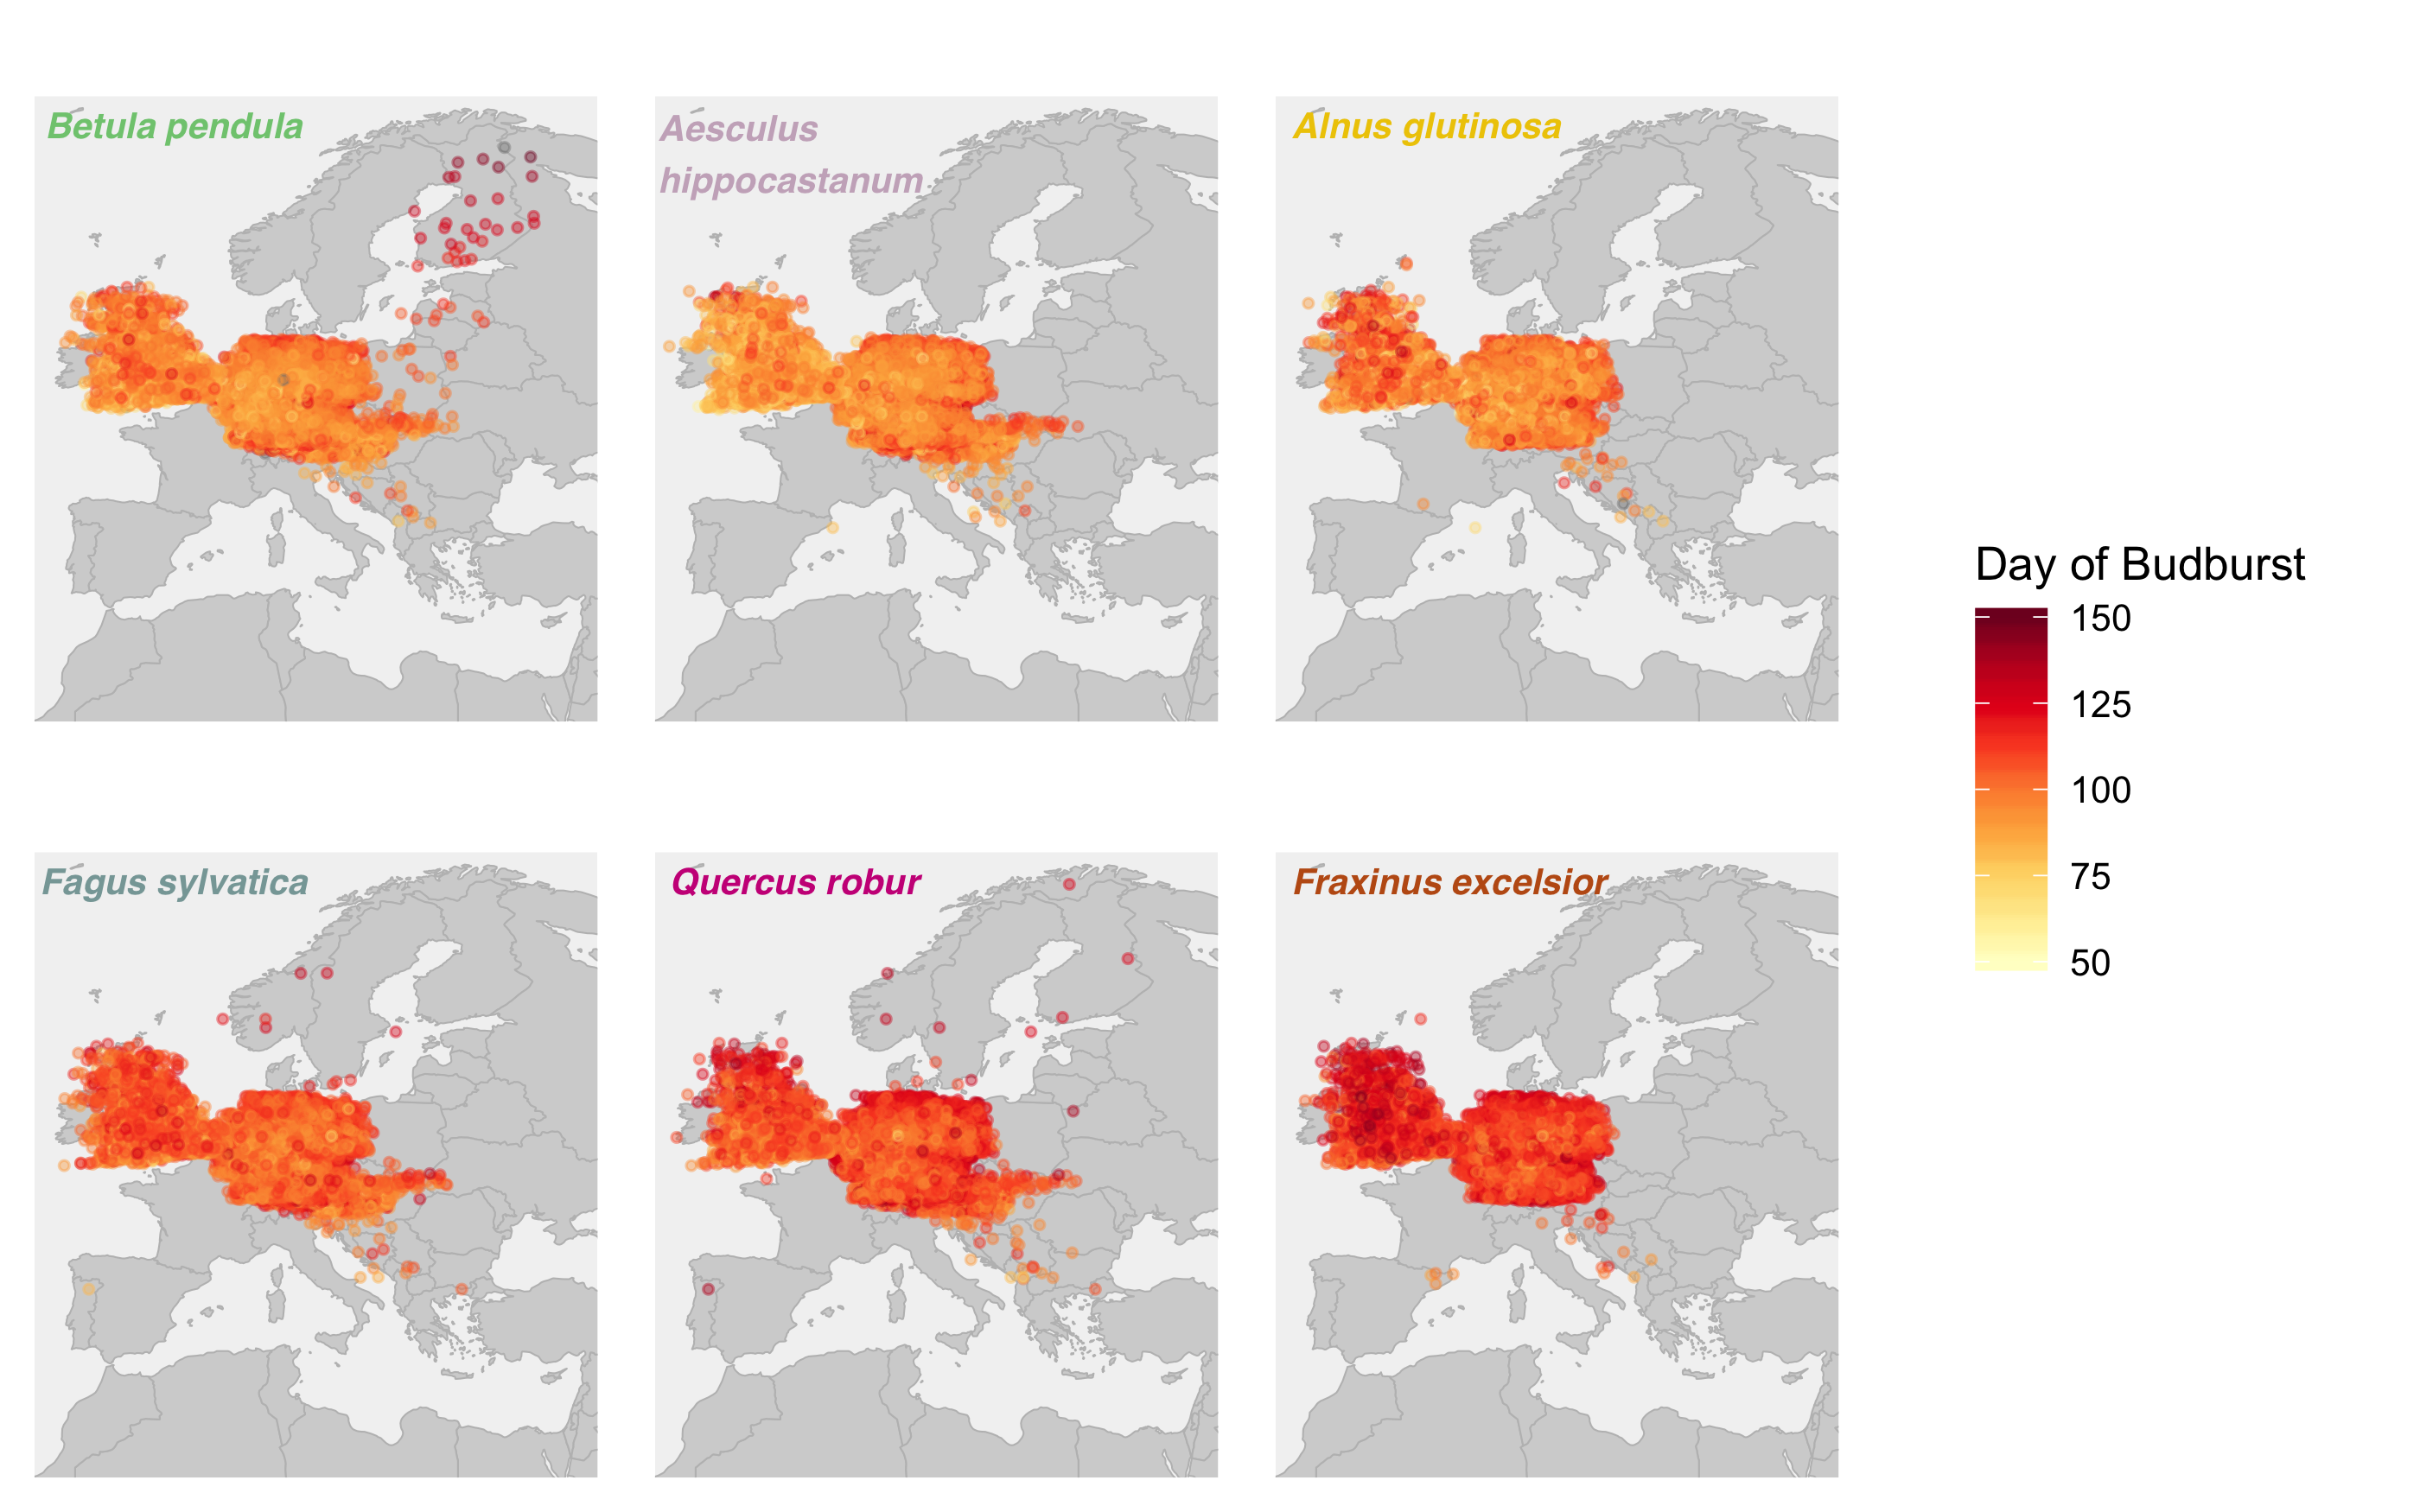
\includegraphics[width=14cm]{..//analyses/figures/BB_base.png}
  -\caption{The average day of budburst is mapped by site for each species. Species are ordered by day of budburst starting with \textit{Betula pendula} as the earliest budburst date to \textit{Fraxinus excelsior}. Earlier budburst dates are yellow and later budburst dates are in red. }\label{fig:bbmap}
  -\end{center}
  -\end{figure}}
  
{\begin{figure} [H]
  -\begin{center}
  -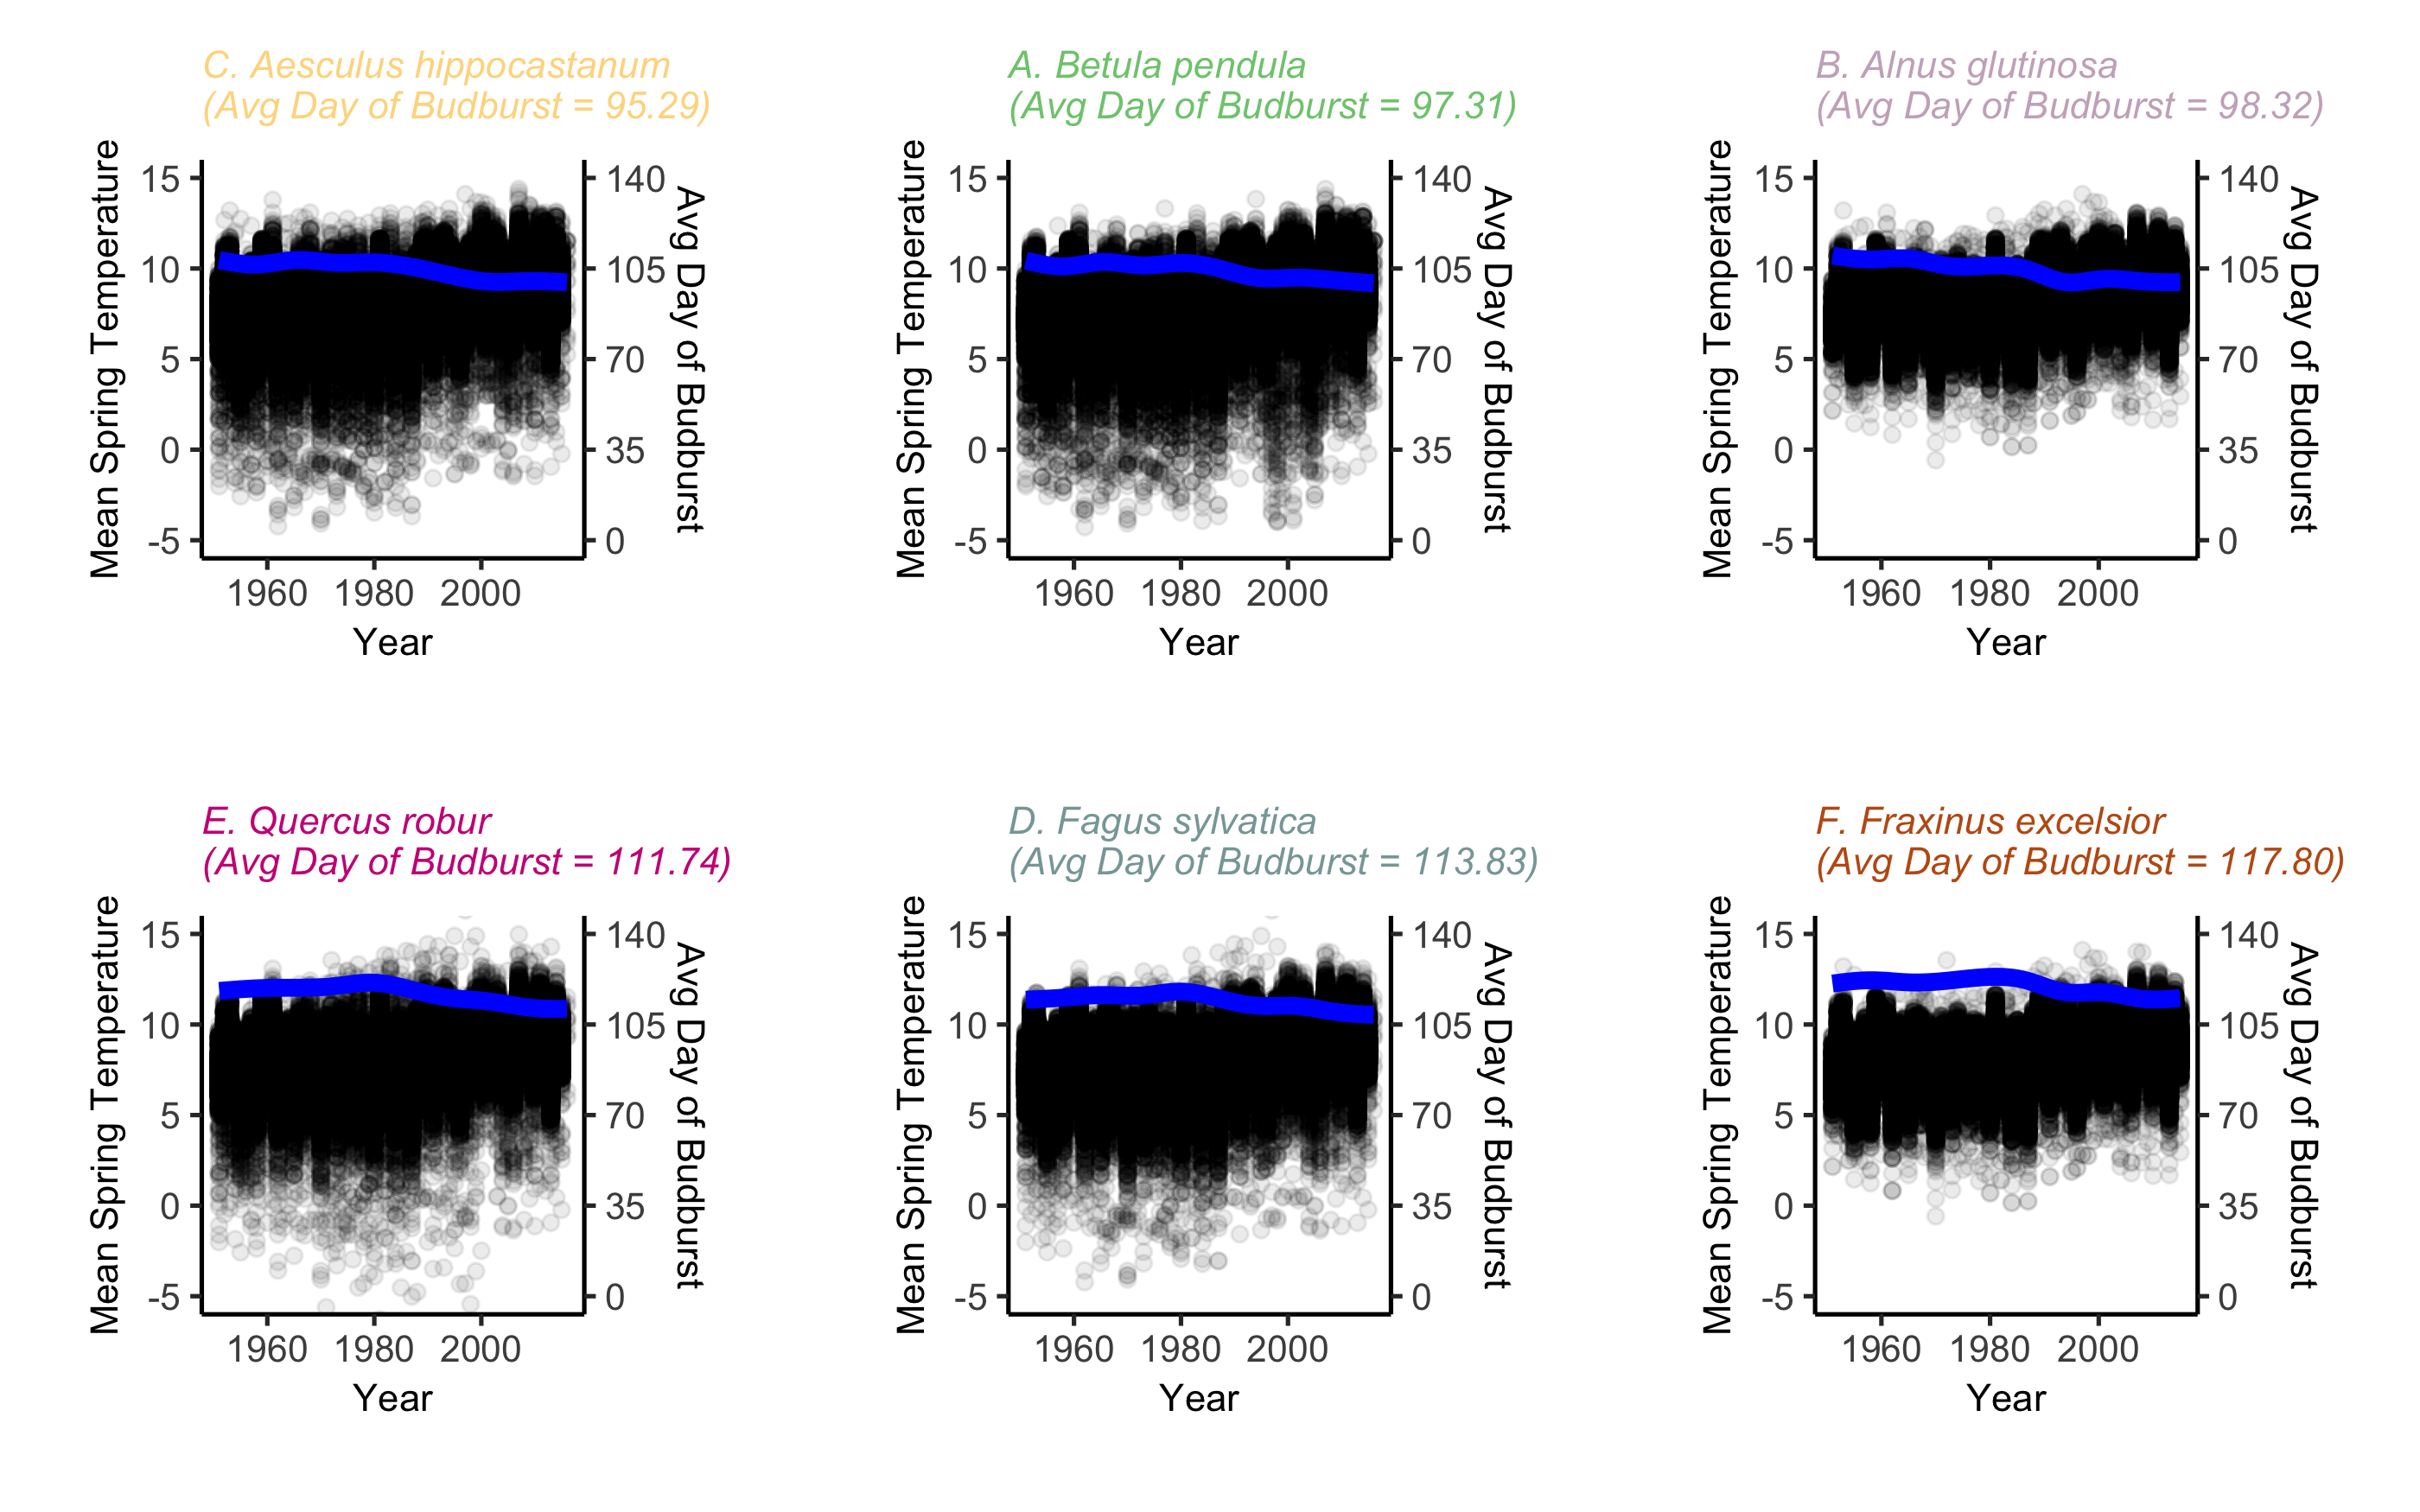
\includegraphics[width=16cm]{..//analyses/figures/MSTBB_bySpp.png}
  -\caption{Mean spring temperatures are plotted for each site over time (from 1951-2016) for each species. The blue line is a smoothing spline, indicating the trend of average day of budburst for each year for each species. Species are ordered by average day of budburst, with the earliest being \textit{Betula pendula} and the latest being \textit{Fraxinus excelsior}. }\label{fig:mst}
  -\end{center}
  -\end{figure}}
  
{\begin{figure} [H]
  -\begin{center}
  -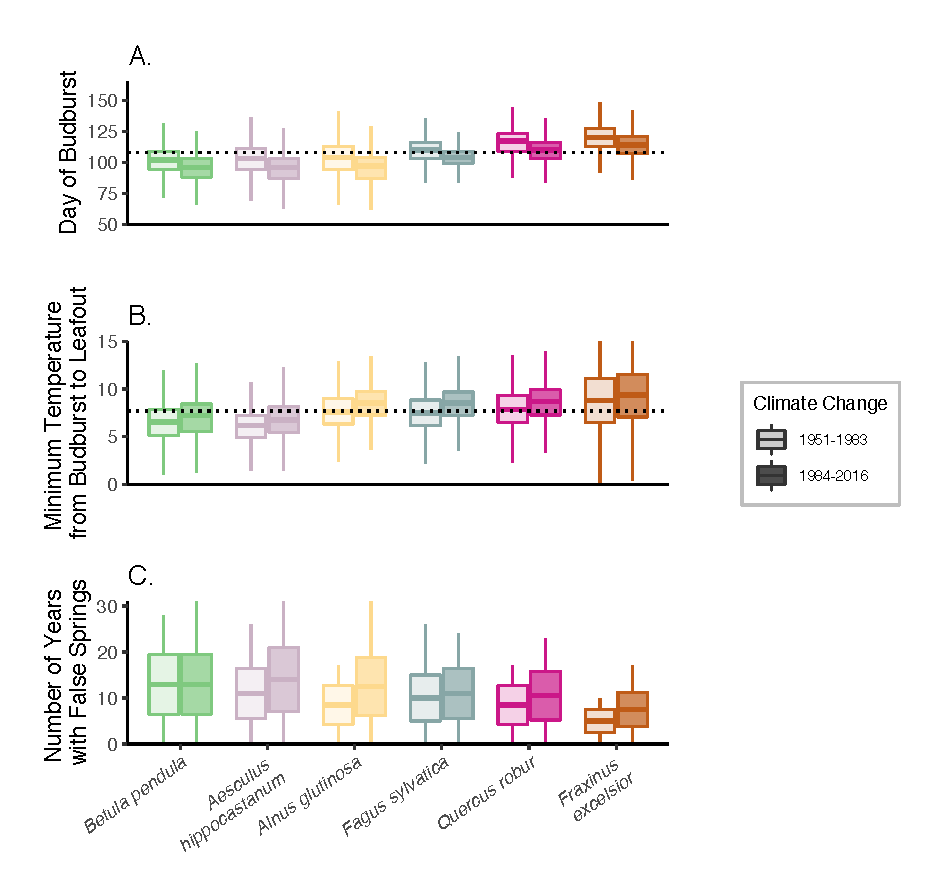
\includegraphics[width=14cm]{..//analyses/figures/Boxplot_BBTminFS_noDots.pdf}
  -\caption{Budburst, minimum temperatures and false springs were compared before and after 1983 for each species. We plotted the day of budburst (A.) before and after 1983 for each species across all sites. We then compared the average minimum temperatures (B.) between budburst and leafout for all species across all sites. The bottom panel (C.), shows the total number of years there was a false spring before and after 1983 at each site across all species. Species are ordered by day of budburst.  }\label{fig:boxfs}
  -\end{center}
  -\end{figure}}
  
  
{\begin{figure} [H]
  -\begin{center}
  -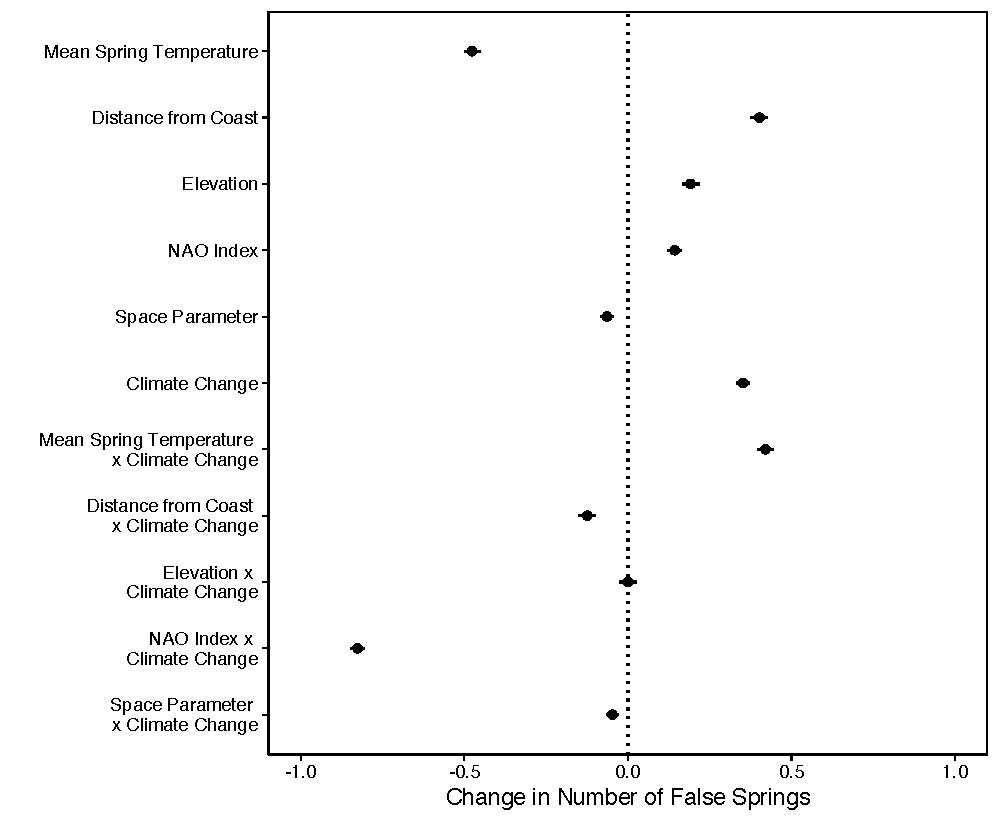
\includegraphics[width=10cm]{..//analyses/figures/model_output_90.pdf}
  -\caption{Model output with standardized durations of vegetative risk for each species. More positive parameter effects indicate an increased probability of a false spring whereas more negative effects suggest a lower probability of a false spring. Uncertainly intervals are at 90\%. Parameter effects closer to zero have less of an effect on false springs. There were 582,211 zeros and 172,877 ones for false spring in the data.}\label{fig:maineffects}
  -\end{center}
  -\end{figure}}


%{\begin{figure} [H]
 % -\begin{center}
  %-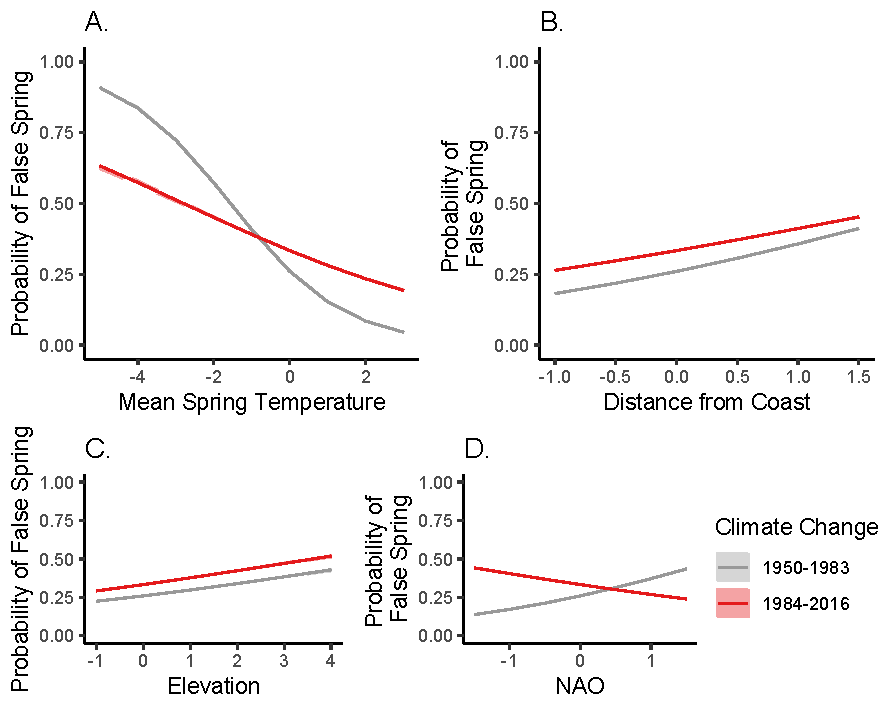
\includegraphics[width=16cm]{..//figures/InteractionPlots/IntrxnPlots_orig.pdf}
  %-\caption{Plots showing the interaction effects on false spring risk for each predictor coupled with climate change. (A.) As mean spring temperature increases, there were fewer false springs but there were fewer false springs after 1983 at sites with lower mean spring temperatures.  (B.) There were more false springs further from the coast and the rate of increase was consistent, however, there were fewer false springs in total after 1983. (C.) As elevation increased, false spring risk increased but the relationship remained consistent after 1983. (D.) As NAO indices increased, there were more false springs before 1983 but fewer after 1983. Since we found the z-score for each predictor, the x-axis for each panel does not reflect the raw data.}\label{fig:intrxns}
  %-\end{center}
  %-\end{figure}}
  
{\begin{figure} [H]
  -\begin{center}
  -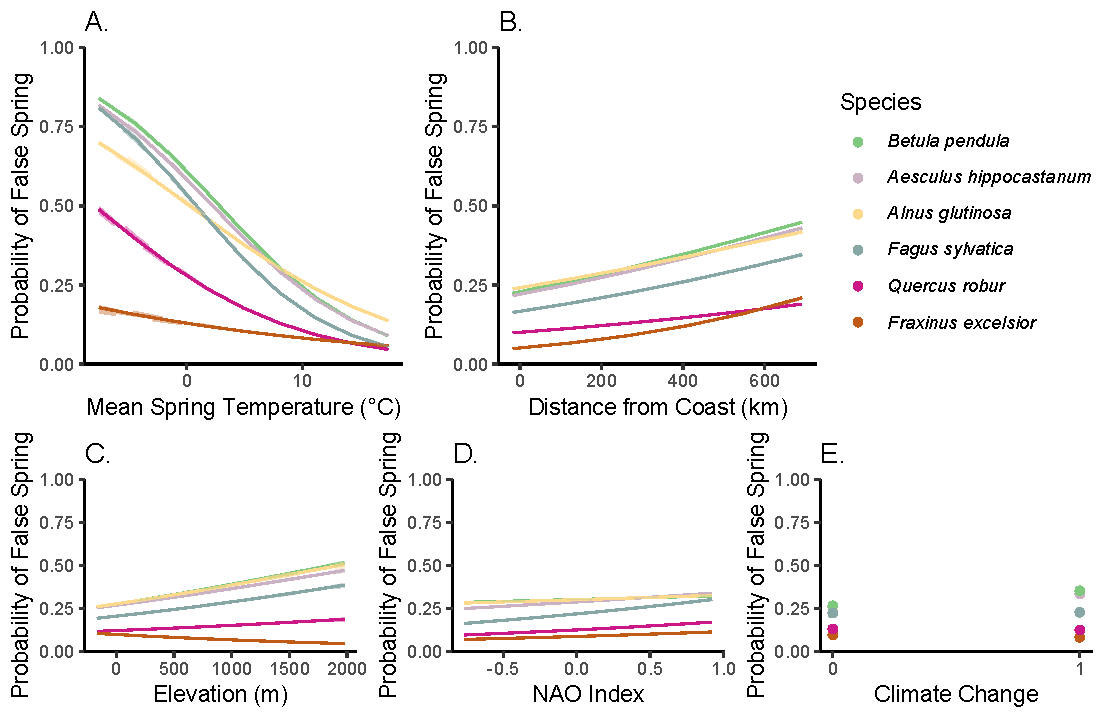
\includegraphics[width=16cm]{..//analyses/figures/InteractionPlots/Species_orig.pdf}
  -\caption{Plots showing the interaction effects of each predictor with species. (A.) As mean spring temperature increases, the probability of a false spring decreases for each species but \textit{Fraxinus excelsior} always has the lowest risk of false spring. (B.) There's an increase in false spring risk for individuals further from the coast, especially for \textit{Fraxinus excelsior}. (C.) The risk of a false spring increases with increasing elevation but the relationship is strongest for \textit{Aesculus hippocastanum} and \textit{Betula pendula}. (D.) There are slightly more false springs in years with higher NAOs, especially for \textit{Fagus sylvatica}.  (E.) There are more false springs after 1983, especially for \textit{Aesculus hippocastanum} and \textit{Betula pendula}. Since we found the z-score for each predictor, the x-axis for each panel does not reflect the raw data.}\label{fig:spp}
  -\end{center}
  -\end{figure}}


  



\end{document}
